%=============================================================================
% PREDIA — Plataforma Clínica Inteligente para la Detección Temprana
%          de Diabetes
% Reporte de Proyecto Integrador
% Universidad Politécnica de Querétaro
%=============================================================================

\documentclass[12pt, letterpaper, twoside]{report}

%-----------------------------------------------------------------------------
% PAQUETES
%-----------------------------------------------------------------------------
\usepackage[spanish, es-tabla]{babel}
\usepackage[utf8]{inputenc}
\usepackage[T1]{fontenc}
\usepackage{lmodern}
\usepackage{microtype}
\emergencystretch=3em

% Geometría — márgenes tipo tesis
\usepackage[
  top=2.5cm, bottom=2.5cm,
  inner=3cm, outer=2.5cm,
  headheight=15pt
]{geometry}

% Tipografía — serif para cuerpo (Times), sans-serif para títulos
\usepackage{mathptmx}        % Times para cuerpo y matemáticas
\usepackage{helvet}           % Helvetica para sans-serif
\renewcommand{\familydefault}{\rmdefault}

% Paleta monocromática
\usepackage[dvipsnames,table]{xcolor}
\definecolor{chapGray}{gray}{0.15}     % Títulos de capítulo (casi negro)
\definecolor{secGray}{gray}{0.25}      % Títulos de sección
\definecolor{subGray}{gray}{0.40}      % Subsecciones y acentos
\definecolor{ruleGray}{gray}{0.50}     % Filetes y líneas
\definecolor{lightGray}{gray}{0.93}    % Fondos suaves (tablas, cajas)
\definecolor{midGray}{gray}{0.65}      % Texto secundario (encabezados)

% Gráficos
\usepackage{graphicx}
\usepackage{float}
\usepackage{wrapfig}

% Tablas — estilo booktabs limpio
\usepackage{booktabs}
\usepackage{tabularx}
\usepackage{multirow}
\usepackage{array}
\usepackage{longtable}
\renewcommand{\arraystretch}{1.35}

% Encabezados y pies de página
\usepackage{fancyhdr}
\usepackage{emptypage}

% Secciones y TOC
\usepackage{titlesec}
\usepackage{titletoc}
\usepackage[titles]{tocloft}

% Hipervínculos — negro para impresión
\usepackage[
  colorlinks=true,
  linkcolor=black,
  urlcolor=black,
  citecolor=black,
  pdftitle={PREDIA — Reporte de Proyecto Integrador},
  pdfauthor={Giannoccaro, Soriano, Álvarez, Muñoz, Villafuerte},
  pdfsubject={Ingeniería en Sistemas Computacionales},
  pdfkeywords={diabetes, machine learning, salud digital, Next.js}
]{hyperref}

% Cajas sobrias
\usepackage{tcolorbox}
\tcbuselibrary{skins, breakable, theorems}

% Código fuente — estilo sobrio
\usepackage{listings}
\lstset{
  basicstyle=\small\ttfamily,
  breaklines=true,
  frame=single,
  rulecolor=\color{ruleGray},
  backgroundcolor=\color{lightGray},
  commentstyle=\color{subGray},
  keywordstyle=\bfseries,
}

% Bibliografía
\usepackage[numbers,sort&compress]{natbib}

% Misceláneos
\usepackage{amsmath, amssymb}
\usepackage{enumitem}
\usepackage{setspace}
\usepackage{caption}
\usepackage{subcaption}
\usepackage{pdfpages}
\usepackage{etoolbox}
\usepackage{needspace}
\usepackage{afterpage}

%-----------------------------------------------------------------------------
% CONFIGURACIÓN DE PÁRRAFOS — estilo tesis con sangría
%-----------------------------------------------------------------------------
\setlength{\parindent}{1.25cm}
\setlength{\parskip}{0pt plus 1pt}
\onehalfspacing

% Prevenir líneas huérfanas y viudas
\widowpenalty=10000
\clubpenalty=10000
\brokenpenalty=10000
\interlinepenalty=10000
\raggedbottom
\predisplaypenalty=10000
\postdisplaypenalty=0

%-----------------------------------------------------------------------------
% ESTILOS DE CAPÍTULOS Y SECCIONES — diseño académico limpio
%-----------------------------------------------------------------------------
\titleformat{\chapter}[display]
  {\normalfont\sffamily\bfseries\color{chapGray}}
  {\Large\MakeUppercase{\chaptertitlename}\ \thechapter}
  {6pt}
  {\noindent\rule{\linewidth}{0.8pt}\endgraf\vspace{4pt}\LARGE}
  [\vspace{4pt}\noindent\rule{\linewidth}{0.4pt}]

\titleformat{name=\chapter, numberless}[display]
  {\normalfont\sffamily\bfseries\color{chapGray}}
  {}
  {0pt}
  {\noindent\rule{\linewidth}{0.8pt}\endgraf\vspace{4pt}\LARGE}
  [\vspace{4pt}\noindent\rule{\linewidth}{0.4pt}]

\titlespacing*{\chapter}{0pt}{0pt}{24pt}

\titleformat{\section}
  {\normalfont\sffamily\Large\bfseries\color{secGray}\raggedright}
  {\thesection}
  {0.8em}
  {}
  [\vspace{2pt}\endgraf\noindent{\color{ruleGray}\rule{\linewidth}{0.4pt}}]

\titleformat{\subsection}
  {\normalfont\sffamily\large\bfseries\color{secGray}}
  {\thesubsection}
  {0.7em}
  {}

\titleformat{\subsubsection}
  {\normalfont\sffamily\normalsize\bfseries\color{subGray}}
  {\thesubsubsection}
  {0.6em}
  {}

\titlespacing*{\section}{0pt}{20pt}{10pt}
\titlespacing*{\subsection}{0pt}{14pt}{6pt}
\titlespacing*{\subsubsection}{0pt}{10pt}{4pt}

% Evitar que secciones queden al final de página sin cuerpo
\newcommand{\sectionbreak}{\needspace{8\baselineskip}}
%-----------------------------------------------------------------------------
% ENCABEZADOS Y PIES DE PÁGINA — minimalista
%-----------------------------------------------------------------------------
\pagestyle{fancy}
\fancyhf{}
\fancyhead[LE]{\small\itshape\color{midGray}\leftmark}
\fancyhead[RO]{\small\itshape\color{midGray}\rightmark}
\fancyfoot[LE,RO]{\small\thepage}
\renewcommand{\headrulewidth}{0.4pt}
\renewcommand{\footrulewidth}{0pt}
\renewcommand{\headrule}{\color{ruleGray}\hrule width\headwidth height\headrulewidth}

% Redefinir estilo plain para las páginas de inicio de capítulo
\fancypagestyle{plain}{
  \fancyhf{}
  \fancyfoot[LE,RO]{\small\thepage}
  \renewcommand{\headrulewidth}{0pt}
}

%-----------------------------------------------------------------------------
% TABLA DE CONTENIDOS — limpia, monocromática
%-----------------------------------------------------------------------------
\setlength{\cftbeforetoctitleskip}{0pt}
\renewcommand{\cfttoctitlefont}{\normalfont\sffamily\huge\bfseries\color{chapGray}}
\renewcommand{\cftchapfont}{\sffamily\bfseries}
\renewcommand{\cftsecfont}{\sffamily}
\renewcommand{\cftsubsecfont}{\sffamily\small}
\renewcommand{\cftchapleader}{\cftdotfill{\cftdotsep}}
\setlength{\cftbeforechapskip}{6pt}

%-----------------------------------------------------------------------------
% CAPTIONS — sobrias
%-----------------------------------------------------------------------------
\captionsetup{
  font={small},
  labelfont={bf},
  labelsep=period,
  skip=8pt
}

%-----------------------------------------------------------------------------
% ENTORNOS PERSONALIZADOS — estilo monocromático
%-----------------------------------------------------------------------------
\newtcolorbox{infobox}[1][]{
  enhanced, breakable,
  colback=lightGray, colframe=ruleGray,
  boxrule=0.5pt, arc=2pt,
  left=10pt, right=10pt, top=8pt, bottom=8pt,
  fontupper=\small,
  title={#1},
  fonttitle=\bfseries\sffamily\color{chapGray},
  coltitle=chapGray,
  colbacktitle=lightGray
}

\newtcolorbox{flowbox}[1][Flujo]{
  enhanced, breakable,
  colback=lightGray, colframe=chapGray,
  boxrule=0.5pt, arc=2pt,
  left=10pt, right=10pt, top=8pt, bottom=8pt,
  fontupper=\small,
  title={\sffamily\bfseries #1},
  attach boxed title to top left={yshift=-2mm, xshift=8mm},
  boxed title style={colback=chapGray, arc=2pt, boxrule=0pt},
  coltitle=white
}

%-----------------------------------------------------------------------------
% COMANDOS AUXILIARES — tablas monocromáticas
%-----------------------------------------------------------------------------
\newcommand{\thead}[1]{\textbf{\sffamily #1}}
\newcommand{\trow}{}

%=============================================================================
\begin{document}
%=============================================================================

%-----------------------------------------------------------------------------
% PORTADA
%-----------------------------------------------------------------------------
\begin{titlepage}
  \thispagestyle{empty}

  \begin{center}
    \vspace*{1cm}

    % Logo UPQ
    
\includegraphics[height=3.2cm]{img/UPQ-Logo.png}\\[0.5cm]

    {\sffamily\large Universidad Politécnica de Querétaro}\\[0.1cm]
    {\sffamily\normalsize Ingeniería en Sistemas Computacionales}\\[2cm]

    {\color{ruleGray}\rule{0.7\linewidth}{0.8pt}}\\[2cm]

    % Logo PREDIA
    
\includegraphics[height=3.5cm]{img/predia-logo.png}\\[0.8cm]

    {\sffamily\Huge\bfseries PREDIA}\\[0.3cm]
    {\sffamily\large Plataforma Clínica Inteligente para la\\
     Detección Temprana de Diabetes}\\[1cm]

    {\color{ruleGray}\rule{0.5\linewidth}{0.4pt}}\\[1.2cm]

    {\sffamily\normalsize\bfseries REPORTE DE PROYECTO INTEGRADOR}\\[0.4cm]
    {\sffamily\normalsize Programa Educativo: Ingeniería en Sistemas Computacionales}\\[2cm]

    % Autores
    {\sffamily\small\bfseries\MakeUppercase{Presenta}}\\[0.4cm]
    \begin{tabular}{c}
      {\sffamily Giannoccaro Quiñonez Arianna Valentina}\\[2pt]
      {\sffamily Soriano Vega Elena Tatiana}\\[2pt]
      {\sffamily Álvarez Sánchez Guillermo}\\[2pt]
      {\sffamily Muñoz Prado Cristopher Yanhyu}\\[2pt]
      {\sffamily Villafuerte Armenta Gabriel Iván}
    \end{tabular}\\[1.5cm]

    % Asesores
    {\sffamily\small\bfseries\MakeUppercase{Asesor UPQ}}\\[0.3cm]
    {\sffamily\small José Javier Moya Moya \quad|\quad Jairo Pacindo Piña}\\[2cm]

    {\color{ruleGray}\rule{0.4\linewidth}{0.4pt}}\\[0.4cm]
    {\sffamily\small El Marqués, Querétaro \quad|\quad Abril 2026}
  \end{center}
\end{titlepage}

%-----------------------------------------------------------------------------
% PÁGINAS PRELIMINARES
%-----------------------------------------------------------------------------
\cleardoublepage
\pagenumbering{roman}

%--- Resumen ------------------------------------------------------------------
\cleardoublepage
\phantomsection
\addcontentsline{toc}{chapter}{Resumen}
\chapter*{Resumen}

El presente proyecto integrador documenta el desarrollo de \textit{Predia} (Plataforma Clínica Inteligente para la Detección Temprana de Diabetes), un sistema integral orientado a la gestión de historiales médicos que incorpora técnicas de Inteligencia Artificial para la estimación del riesgo de diabetes tipo~2. La plataforma permite a profesionales de la salud administrar información clínica y obtener predicciones preventivas mediante un entorno seguro y escalable, construido sobre tecnologías web modernas y una base de datos relacional.

El componente predictivo se sustenta en un modelo de \textit{Machine Learning} entrenado con un conjunto de 757 muestras clínicas, con el que se obtuvo una exactitud del 97.89\% en el conjunto de prueba. No obstante, el tamaño reducido de la muestra exige cautela al generalizar estos resultados a poblaciones diferentes. La arquitectura del sistema se basa en una API RESTful complementada con autenticación mediante JWT y control de acceso por roles (administrador, médico y enfermero). La consistencia entre los entornos de desarrollo y despliegue se garantiza mediante la contenedorización con Docker y la orquestación de servicios con Docker Compose.

La información clínica sensible se organiza mediante un modelo de datos relacional que abarca registros médicos, estudios de laboratorio, mediciones no invasivas y registros de auditoría, lo cual asegura tanto la trazabilidad como la seguridad de los datos. El análisis de factibilidad económica respalda la viabilidad del proyecto, con un retorno de inversión favorable y un periodo de recuperación estimado en menos de dos años.

El mercado objetivo comprende instituciones de salud en México interesadas en la prevención de la diabetes y en la incorporación de tecnologías predictivas. En su conjunto, el proyecto demuestra la aplicabilidad de la Inteligencia Artificial y la ingeniería de software en el abordaje de problemáticas de salud pública, con el fin de favorecer la detección oportuna y contribuir a la mejora de la atención clínica.

\bigskip
\noindent\textbf{Palabras clave:} Inteligencia artificial, aprendizaje automático, plataforma clínica, detección temprana, diabetes tipo~2, apoyo a la toma de decisiones clínicas.

%--- Abstract -----------------------------------------------------------------
\cleardoublepage
\phantomsection
\addcontentsline{toc}{chapter}{Abstract}
\chapter*{Abstract}

This integrative project documents the development of \textit{Predia} (Plataforma Clínica Inteligente para la Detección Temprana de Diabetes), an integrated platform for clinical record management that incorporates Artificial Intelligence for early risk estimation of Type~2 diabetes. The system enables healthcare professionals to securely manage clinical information and obtain preventive risk assessments through a scalable, role-based web platform.

The predictive component relies on a Machine Learning model trained on a dataset of 757 clinical samples, achieving a test-set accuracy of 97.89\%. However, the limited sample size warrants caution when generalizing these results to broader populations. The platform is built on a RESTful API architecture with JWT-based authentication and role-based access control for administrators, physicians, and nursing staff. Containerization through Docker and Docker Compose ensures consistency across development and deployment environments.

Sensitive clinical data is organized through a relational database model encompassing medical records, laboratory studies, anthropometric measurements, and audit logs, thereby ensuring data integrity and traceability. An economic feasibility analysis confirms the viability of the project, demonstrating a favorable return on investment within an estimated recovery period of less than two years.

This project demonstrates the practical applicability of Artificial Intelligence and software engineering in addressing public health challenges, with the aim of supporting early detection and contributing to improved clinical care.

\bigskip
\noindent\textbf{Keywords:} Artificial intelligence, machine learning, clinical platform, early detection, type~2 diabetes, clinical decision support.

%--- Tabla de contenidos ------------------------------------------------------
\tableofcontents

\cleardoublepage
\phantomsection
\addcontentsline{toc}{chapter}{\listfigurename}
\listoffigures

\cleardoublepage
\phantomsection
\addcontentsline{toc}{chapter}{\listtablename}
\listoftables

%=============================================================================
\cleardoublepage
\pagenumbering{arabic}
%=============================================================================

%=============================================================================
\chapter{Antecedentes}
%=============================================================================

\section*{Tema de proyecto}
\addcontentsline{toc}{section}{Tema de proyecto}

\begin{figure}[htbp]
  \centering
  
\includegraphics[width=0.35\linewidth]{img/predia-logo.png}
  \caption{Logo del proyecto PREDIA.}
  \label{fig:logo_predia}
\end{figure}

%------------------------------------------------------------------------------
\section{Contexto del problema}
%------------------------------------------------------------------------------

La diabetes mellitus tipo~2 constituye uno de los principales desafíos de salud pública tanto en México como a nivel mundial. De acuerdo con la Federación Internacional de Diabetes (IDF), México ocupa el sexto lugar global en prevalencia de esta enfermedad, con aproximadamente 13.6 millones de personas diagnosticadas en 2024. Las complicaciones asociadas ---enfermedades cardiovasculares, neuropatías, retinopatías y nefropatías--- generan costos significativos para los sistemas de salud y deterioran la calidad de vida de los pacientes.

Un problema recurrente en el sistema de salud mexicano radica en el diagnóstico tardío de esta enfermedad: un porcentaje considerable de pacientes recibe su diagnóstico cuando la condición ya ha progresado de forma sustancial, lo cual limita las opciones terapéuticas y eleva el riesgo de complicaciones graves. En este contexto, la detección temprana mediante el análisis sistemático de factores de riesgo clínicos resulta esencial para posibilitar intervenciones preventivas que mejoren el pronóstico de los pacientes. Este escenario epidemiológico motiva, a su vez, la búsqueda de soluciones tecnológicas que apoyen la labor clínica.

%------------------------------------------------------------------------------
\section{Gestión de historiales médicos}
%------------------------------------------------------------------------------

En el ámbito de la gestión clínica, un número considerable de instituciones de salud en México operan aún con sistemas de expedientes físicos o plataformas digitales desconectadas entre sí. Esta fragmentación dificulta el seguimiento longitudinal de los pacientes, la identificación de patrones de riesgo y la toma de decisiones fundamentadas en evidencia. La ausencia de integración entre los distintos sistemas genera silos de información que impiden construir una visión integral del estado de salud de cada paciente.

Esta problemática se agrava cuando se considera la necesidad de alimentar herramientas predictivas con datos clínicos estructurados y consistentes. Sin una plataforma que centralice la información médica, la aplicación de técnicas de Inteligencia Artificial al ámbito clínico permanece limitada, pues los modelos predictivos requieren conjuntos de datos organizados, validados y accesibles en tiempo real.

%------------------------------------------------------------------------------
\section{Inteligencia Artificial en la medicina preventiva}
%------------------------------------------------------------------------------

En los últimos años, la aplicación de Inteligencia Artificial y \textit{Machine Learning} en el sector salud ha producido resultados prometedores. Diversos estudios han evidenciado que los modelos predictivos pueden identificar pacientes en riesgo de desarrollar diabetes tipo~2 con exactitudes superiores al 85\%, empleando variables clínicas accesibles como glucosa en ayunas, índice de masa corporal, presión arterial e historial familiar.

Investigaciones previas han explorado algoritmos de predicción de diabetes mediante técnicas como regresión logística, árboles de decisión, \textit{random forests} y redes neuronales. No obstante, gran parte de estas soluciones permanecen circunscritas al ámbito académico, ya que no se han traducido en herramientas directamente utilizables por los profesionales de salud en su práctica clínica. Entre las razones de esta brecha se encuentran la complejidad de integrar los modelos en flujos de trabajo médicos existentes, las limitaciones de los conjuntos de datos disponibles ---frecuentemente reducidos o sesgados--- y la ausencia de plataformas clínicas que actúen como vehículo de estas capacidades predictivas.

%------------------------------------------------------------------------------
\section{Tecnologías de virtualización en desarrollo de software}
%------------------------------------------------------------------------------

La adopción de tecnologías de contenedores, y en particular Docker, ha transformado de manera significativa el desarrollo de software en el sector salud. La contenedorización permite encapsular cada componente de una aplicación ---junto con sus dependencias, configuraciones y variables de entorno--- en unidades aisladas y reproducibles, lo cual garantiza un comportamiento idéntico en los entornos de desarrollo, pruebas y producción.

Esta característica resulta particularmente crítica en aplicaciones médicas, donde la precisión y la confiabilidad del software inciden directamente en la seguridad del paciente. Un modelo de \textit{Machine Learning}, por ejemplo, puede producir resultados distintos si las versiones de las bibliotecas numéricas difieren entre entornos; la contenedorización elimina esta fuente de variabilidad. Adicionalmente, herramientas de orquestación como Docker Compose facilitan el despliegue coordinado de arquitecturas multicapa ---frontend, backend, base de datos y servicios auxiliares--- mediante un único archivo de configuración declarativo, reduciendo la complejidad operativa y los errores de configuración manual.

%------------------------------------------------------------------------------
\section{Necesidad del proyecto}
%------------------------------------------------------------------------------

Los antecedentes expuestos ---la carga epidemiológica de la diabetes en México, las deficiencias en la gestión de historiales clínicos, el potencial aún no explotado de la IA en entornos clínicos reales y las ventajas de la contenedorización para software médico--- convergen en la necesidad de una plataforma que articule gestión de información clínica con capacidades predictivas de Inteligencia Artificial. En este contexto surge Predia, concebida como una solución accesible para profesionales de salud y construida sobre tecnologías modernas que favorezcan la escalabilidad, la seguridad y la mantenibilidad del sistema. Su propósito central consiste en reducir la distancia entre la investigación académica en IA médica y las herramientas que los clínicos pueden emplear en su práctica cotidiana, contribuyendo así a la medicina preventiva.

%=============================================================================
\chapter{Marco Teórico}
%=============================================================================

El marco teórico que se presenta a continuación establece los pilares conceptuales, tecnológicos y científicos sobre los que se sustenta \textbf{PREDIA}. Como se expuso en el capítulo de antecedentes, la convergencia entre la carga epidemiológica de la diabetes, las deficiencias en la gestión de información clínica y el potencial inexplotado de la Inteligencia Artificial en entornos médicos reales justifica el desarrollo de una plataforma que integre ambas dimensiones. El sistema resultante no se limita a la predicción del riesgo; ofrece una solución clínica integral que abarca la gestión de pacientes, el seguimiento del historial médico, la generación de recetas y la explotación de algoritmos de aprendizaje automático para estimar la probabilidad de desarrollo de la enfermedad.

Los fundamentos teóricos se articulan desde cuatro perspectivas principales:
\begin{enumerate}[leftmargin=2cm]
  \item la \textbf{epidemiología de la diabetes};
  \item los \textbf{fundamentos del Machine Learning aplicado en salud};
  \item las \textbf{arquitecturas de software modernas}; y
  \item los \textbf{estándares de seguridad en sistemas médicos digitales}.
\end{enumerate}
Cada sección fundamenta las decisiones de diseño y tecnología adoptadas en el proyecto.

%------------------------------------------------------------------------------
\section{Diabetes mellitus: contexto epidemiológico}
%------------------------------------------------------------------------------

\subsection{Definición y clasificación}

La \textbf{Diabetes Mellitus (DM)} es un grupo de enfermedades metabólicas caracterizadas por una hiperglucemia crónica que resulta de defectos en la secreción de insulina, en la acción de la insulina, o en ambos procesos simultáneamente. La Organización Mundial de la Salud (OMS) clasifica la diabetes en tres tipos principales (Tabla~\ref{tab:clasificacion_dm}).

\begin{table}[H]
  \centering
  \caption{Clasificación de la Diabetes Mellitus según la OMS.}
  \label{tab:clasificacion_dm}
  \begin{tabularx}{\linewidth}{>{\bfseries\sffamily}l X c}
    \toprule
    \thead{Tipo} & \thead{Descripción} & \thead{Prevalencia} \\
    \midrule
    \trow Tipo 1 (DM1) & Enfermedad autoinmune; destrucción de células beta del páncreas. Requiere insulina exógena. & 5--10\% \\
    Tipo 2 (DM2) & Resistencia insulínica y/o insuficiencia de producción. Diana principal del modelo predictivo. & 90--95\% \\
    \trow Gestacional & Se desarrolla durante el embarazo. Riesgo alto de complicaciones materno-fetales y DM2 futura. & Variable \\
    \bottomrule
  \end{tabularx}
\end{table}

\subsection{Factores de riesgo}

La predicción temprana de la diabetes tipo~2 depende del análisis de un conjunto de \textbf{factores de riesgo} ampliamente documentados en la literatura médica. Estos factores se dividen en variables modificables y no modificables, y constituyen las características de entrada del modelo de Machine Learning implementado en PREDIA (Tabla~\ref{tab:factores_riesgo}).

\begin{table}[H]
  \centering
  \caption{Factores de riesgo para diabetes tipo~2 y su relevancia predictiva.}
  \label{tab:factores_riesgo}
  \begin{tabularx}{\linewidth}{X l X}
    \toprule
    \thead{Factor de riesgo} & \thead{Categoría} & \thead{Relevancia} \\
    \midrule
    \trow Edad & No modificable & Alta — correlación directa con incidencia \\
    Índice de Masa Corporal (IMC) & Modificable & Muy alta — predictor principal \\
    \trow Historial familiar de diabetes & No modificable & Alta — componente genética 30--70\% \\
    Niveles de glucosa en ayuno & Biológico & Muy alta — indicador clínico directo \\
    \trow Niveles de colesterol & Modificable & Media — factor metabólico asociado \\
    Presión arterial & Modificable & Media — comorbilidad frecuente \\
    \trow Sedentarismo & Modificable & Alta — estilo de vida \\
    Diabetes gestacional previa & No modificable & Alta — predictor femenino específico \\
    \bottomrule
  \end{tabularx}
\end{table}

\subsection{Impacto global}

Según datos de la Federación Internacional de Diabetes (IDF, 2021), aproximadamente \textbf{537 millones de adultos} en todo el mundo padecen diabetes, y se proyecta que la cifra alcance \textbf{783 millones para 2045}. En el caso de México, la prevalencia de diabetes tipo~2 sitúa al país entre los de mayor carga epidemiológica en América Latina, con una proporción de casos no diagnosticados que agrava la problemática. Esta realidad subraya la necesidad urgente de herramientas predictivas accesibles y eficientes, capaces de operar con los datos clínicos disponibles en el contexto mexicano.

%------------------------------------------------------------------------------
\section{Machine Learning en salud}
%------------------------------------------------------------------------------

\subsection{Definición y fundamentos}

El \textbf{Machine Learning (ML)} es una rama de la Inteligencia Artificial que dota a los sistemas informáticos de la capacidad de aprender y mejorar a partir de la experiencia sin estar programados explícitamente para cada tarea. En el contexto de la salud, el ML permite identificar patrones complejos en grandes conjuntos de datos clínicos, facilitando la predicción de enfermedades, el diagnóstico temprano y la personalización de tratamientos.

El aprendizaje automático se divide en tres paradigmas principales: \textbf{aprendizaje supervisado} (enfoque utilizado en PREDIA), donde el modelo se entrena con datos etiquetados; \textbf{aprendizaje no supervisado}, que busca estructuras inherentes en los datos sin etiquetas; y \textbf{aprendizaje por refuerzo}, donde un agente aprende mediante interacción con un entorno.

\subsection{Algoritmos de clasificación aplicables}

Para la tarea de predicción de diabetes —enmarcada como un problema de \textbf{clasificación binaria} (diabético / no diabético)— existen diversos algoritmos candidatos. El modelo implementado fue seleccionado tras un proceso de evaluación comparativa (Tabla~\ref{tab:algoritmos_ml}).

\begin{table}[H]
  \centering
  \caption{Algoritmos de clasificación evaluados para el modelo predictivo de PREDIA.}
  \label{tab:algoritmos_ml}
  \begin{tabularx}{\linewidth}{l l X}
    \toprule
    \thead{Algoritmo} & \thead{Tipo} & \thead{Fortalezas} \\
    \midrule
    \trow Logistic Regression & Lineal & Interpretabilidad alta, rápido de entrenar \\
    Decision Tree & Árbol & Visualizable, maneja variables categóricas \\
    \trow Random Forest & Ensemble & Robusto, reduce sobreajuste, alta precisión \\
    Support Vector Machine & Kernel & Efectivo en alta dimensionalidad \\
    \trow K-Nearest Neighbors & Distancia & Simple, sin fase de entrenamiento explícita \\
    Neural Network & Profundo & Representaciones no lineales complejas \\
    \bottomrule
  \end{tabularx}
\end{table}

\subsection{Métricas de evaluación}

La validación de un modelo predictivo en contextos médicos exige ir más allá de la exactitud (\textit{accuracy}) simple, ya que esta métrica puede resultar engañosa ante clases desbalanceadas. Las métricas complementarias empleadas en PREDIA se describen a continuación. La \textbf{\textit{Precision}} cuantifica la proporción de predicciones positivas que resultan correctas, lo cual es relevante para evitar falsos positivos que generen ansiedad innecesaria en el paciente. El \textbf{\textit{Recall}} (sensibilidad) mide la proporción de casos positivos reales que el modelo identifica correctamente, métrica crítica en contextos médicos donde un falso negativo puede retrasar un diagnóstico. El \textbf{\textit{F1-Score}} es la media armónica entre ambas, especialmente útil cuando las clases están desbalanceadas. Finalmente, el \textbf{área bajo la curva ROC (AUC)} evalúa la capacidad discriminativa global del modelo.

El modelo implementado en PREDIA alcanzó una exactitud del 97.89\% sobre un conjunto de 757 muestras. Si bien este resultado es alentador, debe interpretarse con reservas: el tamaño limitado de la muestra puede propiciar sobreajuste (\textit{overfitting}), y la generalización a poblaciones clínicas más diversas requiere validación adicional con conjuntos de datos independientes.

\subsection{Aplicaciones del ML en medicina}

La inteligencia artificial ha mostrado un potencial transformador en la medicina, con aplicaciones desde el diagnóstico por imágenes hasta la predicción de riesgos cardiovasculares. En el dominio de la diabetes, los modelos predictivos han demostrado capacidad de identificar pacientes en prediabetes años antes del diagnóstico clínico convencional, permitiendo intervenciones preventivas más efectivas. PREDIA se enmarca en esta tendencia, democratizando el acceso a predicción inteligente mediante una interfaz clínica accesible.

%------------------------------------------------------------------------------
\section{Arquitecturas de software modernas}
%------------------------------------------------------------------------------

\subsection{Arquitectura cliente-servidor y API REST}

La arquitectura de \textbf{PREDIA} adopta el patrón \textbf{cliente-servidor} basado en una API RESTful (\textit{Representational State Transfer}). REST, propuesta por Roy Fielding en 2000, define principios arquitectónicos que incluyen comunicación sin estado (\textit{stateless}), representación uniforme de recursos y utilización de métodos HTTP estándar (GET, POST, PUT, DELETE). El proyecto implementa \textbf{24+ endpoints REST}, organizados en recursos semánticos: autenticación, pacientes, agenda, consultas, recetas, signos vitales y predicciones.

\subsection{Next.js y \textit{Server-Side Rendering}}

Next.js es un \textit{framework} de React que soporta múltiples modelos de renderizado: \textit{Server-Side Rendering (SSR)}, \textit{Static Site Generation (SSG)} y \textit{Client-Side Rendering (CSR)}. La elección de Next.js sobre alternativas como Vite o Create React App se fundamentó en tres factores: la posibilidad de implementar \textit{API Routes} que alojan la lógica del backend dentro del mismo proyecto ---simplificando el despliegue y la operación del sistema---, el soporte nativo para SSR que mejora el rendimiento percibido y el SEO, y la integración fluida con el ecosistema de React~19 para la construcción de interfaces declarativas.

\subsection{\textit{Progressive Web Apps} (PWA)}

Las \textbf{Progressive Web Apps} combinan la accesibilidad de las aplicaciones web con funcionalidades nativas de las aplicaciones móviles. Sus características fundamentales incluyen capacidad de funcionamiento \textit{offline} mediante Service Workers, instalabilidad en dispositivos y sincronización automática. Para un entorno clínico como el de PREDIA, estas características son críticas, ya que los profesionales de salud pueden necesitar acceder a datos del paciente en zonas de cobertura limitada.

\begin{infobox}[Sincronización \textit{offline} en contexto clínico]
La arquitectura PWA de PREDIA contempla una estrategia de cola de operaciones pendientes para escenarios sin conectividad. Cuando el dispositivo pierde conexión, las acciones del usuario (registro de consultas, actualización de historial) se almacenan localmente. Al restablecerse la conexión, el sistema ejecuta automáticamente estas operaciones en el orden correcto, resolviendo conflictos mediante una estrategia de \textit{last-write-wins} enriquecida con marcas de tiempo. Cabe señalar que esta funcionalidad se ha implementado a nivel de arquitectura, aunque su validación en condiciones clínicas reales constituye un trabajo pendiente.
\end{infobox}

\subsection{Base de datos relacional y ORM}

El sistema utiliza \textbf{MySQL} como motor de base de datos relacional. El acceso se gestiona mediante \textbf{Prisma}, un ORM de nueva generación que proporciona un cliente \textit{type-safe} generado automáticamente a partir del esquema de la base de datos. El modelo de datos incluye entidades para usuarios y roles, pacientes, historial clínico (antecedentes, alergias, vacunas, patologías), atención médica (consultas, recetas, signos vitales), documentos y el módulo de IA (predicciones y modelos).

%------------------------------------------------------------------------------
\section{Seguridad en sistemas de salud digital}
%------------------------------------------------------------------------------

\subsection{Importancia de la seguridad en datos médicos}

Los datos de salud representan información altamente sensible y personal. A nivel internacional, regulaciones como la \textbf{HIPAA} (Estados Unidos), el \textbf{GDPR} (Europa) y la \textbf{Ley General de Protección de Datos Personales} (México) establecen marcos legales estrictos. Cualquier sistema que maneje datos clínicos debe implementar mecanismos robustos de autenticación, autorización y auditoría.

\subsection{Autenticación con JWT}

Los \textbf{JSON Web Tokens (JWT)} son un estándar abierto (RFC 7519) para crear tokens compactos y seguros. Un JWT consta de tres partes codificadas en Base64: el \textit{header} (algoritmo de firma), el \textit{payload} (datos del usuario y expiración) y la \textit{firma} (verificación de integridad). En PREDIA, los JWT mantienen sesiones autenticadas tras el inicio de sesión, eliminando la necesidad de almacenar estados de sesión en el servidor.

\subsection{Control de acceso basado en roles (RBAC)}

El principio del \textbf{menor privilegio} es fundamental en sistemas médicos. PREDIA implementa un modelo de \textbf{Role-Based Access Control (RBAC)} con tres roles diferenciados (Tabla~\ref{tab:rbac}).

\begin{table}[H]
  \centering
  \caption{Roles y permisos del sistema PREDIA.}
  \label{tab:rbac}
  \begin{tabularx}{\linewidth}{l X c}
    \toprule
    \thead{Rol} & \thead{Permisos principales} & \thead{Nivel} \\
    \midrule
    \trow Administrador & Gestión de usuarios, configuración del sistema, auditoría completa & Total \\
    Médico & Consultas, recetas, predicciones, historial clínico completo & Alto \\
    \trow Enfermero & Signos vitales, agenda, visualización de pacientes & Medio \\
    \bottomrule
  \end{tabularx}
\end{table}

\subsection{Auditoría y trazabilidad}

La \textbf{auditoría completa} implementada en PREDIA registra todas las operaciones realizadas sobre los datos de pacientes. Cada evento auditable incluye la identidad del usuario, la marca de tiempo, el tipo de operación y los datos afectados. Este mecanismo es esencial no solo para cumplir con regulaciones, sino también para investigar incidentes de seguridad y garantizar la integridad de los registros médicos.

%------------------------------------------------------------------------------
\section{Tecnologías complementarias}
%------------------------------------------------------------------------------

\subsection{Reconocimiento de voz (Web Speech API)}

La \textbf{Web Speech API} es una interfaz nativa del navegador que permite la transcripción de habla a texto sin necesidad de servicios externos. En el contexto clínico, el dictado por voz agiliza el registro de notas durante las consultas, permitiendo al médico mantener el contacto visual con el paciente mientras la información se captura automáticamente.

\subsection{TypeScript y validación con Zod}

TypeScript aporta un sistema de tipos estático sobre JavaScript, detectando errores en fase de desarrollo. La biblioteca \textbf{Zod} proporciona validación de datos en tiempo de ejecución mediante esquemas declarativos. En un sistema que maneja datos médicos, la validación es crucial: un valor incorrecto en un campo de presión arterial o nivel de glucosa puede tener consecuencias clínicas relevantes.

\subsection{\textit{Dashboard} médico interactivo}

El concepto de \textbf{dashboard clínico} proviene de la necesidad de presentar información dispersa de forma consolidada y accionable. PREDIA implementa un \textit{dashboard} con \textit{widgets} de signos vitales, acciones rápidas, alertas de riesgo y resumen crítico del paciente, siguiendo los principios de \textbf{diseño centrado en el usuario} (\textit{User-Centered Design}).

%------------------------------------------------------------------------------
\section{Integración del modelo de predicción en el sistema}
%------------------------------------------------------------------------------

La integración del modelo de \textit{Machine Learning} dentro de la plataforma sigue un flujo arquitectónico definido: el modelo predictivo, desarrollado y entrenado en \textbf{Python}, expone sus capacidades a través del \textit{endpoint} \texttt{/api/predicciones/nueva}. El \textit{frontend} captura los datos clínicos del paciente mediante formularios validados, los envía al \textit{backend}, y este invoca al modelo Python para obtener la estimación de riesgo.

Esta separación permite que cada componente evolucione de forma independiente: el modelo puede reentrenarse con nuevos datos sin afectar la interfaz de usuario. Este patrón, conocido como \textbf{desacoplamiento de servicios}, constituye un principio fundamental en arquitecturas orientadas a servicios. No obstante, dicho desacoplamiento introduce consideraciones adicionales, como la latencia inherente a la invocación interprocesal, la necesidad de gestionar errores del servicio Python de manera transparente para el usuario, y la dependencia de que ambos servicios se encuentren operativos simultáneamente.

\begin{flowbox}[Flujo de predicción]
  \begin{enumerate}[leftmargin=1.2cm, topsep=2pt]
    \item El médico ingresa datos del paciente en el formulario del frontend.
    \item Los datos se validan con Zod y se envían al backend vía API REST.
    \item El backend invoca al modelo Python de predicción.
    \item El modelo retorna la probabilidad de diabetes y los factores de riesgo principales.
    \item El resultado se almacena en la base de datos y se presenta en el \textit{dashboard} del paciente.
  \end{enumerate}
\end{flowbox}

%------------------------------------------------------------------------------
\section{Resumen del marco conceptual}
%------------------------------------------------------------------------------

\begin{table}[H]
  \centering
  \caption{Relación entre los pilares teóricos y su función en PREDIA.}
  \label{tab:resumen_marco}
  \begin{tabularx}{\linewidth}{l X c}
    \toprule
    \thead{Pilar teórico} & \thead{Función en el proyecto} & \thead{Sección} \\
    \midrule
    \trow Epidemiología & Justifica la necesidad del sistema y define los factores de riesgo que alimentan al modelo. & §2.1 \\
    Machine Learning & Proporciona la capacidad predictiva (97.89\% de exactitud con 757 muestras) para identificar pacientes en riesgo. & §2.2 \\
    \trow Arquitectura de software & Define la estructura tecnológica: Next.js, REST, MySQL, PWA y sincronización \textit{offline}. & §2.3 \\
    Seguridad & Protege los datos médicos mediante JWT, RBAC y auditoría, cumpliendo regulaciones. & §2.4 \\
    \trow Tecnologías complementarias & Aporta voz, validación y visualización avanzada al entorno clínico. & §2.5 \\
    Integración ML-plataforma & Conecta el modelo ML con la plataforma mediante desacoplamiento de servicios. & §2.6 \\
    \bottomrule
  \end{tabularx}
\end{table}

%=============================================================================
\chapter{Definición del proyecto}
%=============================================================================

%------------------------------------------------------------------------------
\section{Planteamiento del problema}
%------------------------------------------------------------------------------

Como se estableció en el capítulo anterior, la diabetes mellitus tipo~2 representa uno de los desafíos de salud pública más graves en México. Los datos más recientes de la Federación Internacional de Diabetes indican que en 2024 aproximadamente 13.6 millones de personas entre 20 y 79 años padecen esta enfermedad, lo que equivale al 16.4\% de la población adulta en dicho rango de edad \citep{idf_atlas, ogle2025}. Esta cifra supone un incremento significativo respecto a los 12.4 millones de casos registrados en 2022, lo cual evidencia una tendencia creciente que demanda acciones preventivas inmediatas \citep{basto2021}.

La dimensión del problema se agrava al considerar que la diabetes constituye la tercera causa de muerte en el país, y que casi la mitad de los casos permanecen sin diagnosticar, con el consecuente aumento del riesgo de complicaciones graves \citep{basto2021}. Datos recientes revelan que solo el 70\% de las personas con diabetes conocen su condición, y únicamente el 40\% recibe atención médica adecuada \citep{barquera2021}. Esta realidad configura un escenario en el que las herramientas de detección temprana resultan no solo útiles, sino necesarias.

Las deficiencias en la gestión de historiales médicos descritas en los antecedentes ---fragmentación de la información, sistemas desconectados y dificultades para el seguimiento longitudinal--- se suman a la brecha existente entre los avances académicos en IA aplicada a la predicción de diabetes y su disponibilidad como herramientas clínicas prácticas. A pesar de que diversos estudios han demostrado la capacidad de los modelos predictivos para anticipar la enfermedad con hasta un año de antelación respecto a la aparición de síntomas \citep{contreras2018}, la ausencia de plataformas integradas que combinen gestión clínica con capacidades predictivas sigue limitando las oportunidades de intervención preventiva oportuna.

%------------------------------------------------------------------------------
\section{Justificación}
%------------------------------------------------------------------------------

El desarrollo de la plataforma PREDIA se justifica desde múltiples perspectivas complementarias: su impacto potencial en la salud pública, la viabilidad técnica y económica del proyecto, un marco regulatorio favorable, y la necesidad expresada tanto por profesionales de la salud como por la población general. A continuación se detalla cada una de estas dimensiones.

\subsection{Impacto en salud pública}

Con 13.6 millones de personas afectadas por diabetes en México y aproximadamente la mitad sin diagnosticar, existe una necesidad urgente de herramientas que faciliten la detección temprana. La plataforma Predia aborda directamente esta problemática al integrar capacidades de Inteligencia Artificial que pueden identificar pacientes en riesgo antes de que desarrollen diabetes establecida. Según estudios del \textit{Diabetes Prevention Program}, intervenciones preventivas oportunas pueden reducir hasta en un 58\% el riesgo de progresión.

\subsection{Validación de necesidad por usuarios}

La elicitación de requisitos mediante encuestas a 135 personas —incluyendo profesionales de salud y población general— proporciona evidencia sólida de la necesidad del sistema:

\begin{itemize}[leftmargin=1.5cm]
  \item El \textbf{95\%} de los encuestados considera importante tener información comprensible sobre diabetes.
  \item El \textbf{89\%} valora como esencial el acceso a historial clínico completo.
  \item El \textbf{82\%} confía en el uso de Inteligencia Artificial como apoyo en decisiones médicas.
  \item El \textbf{74\%} expresa preocupación por la privacidad de datos médicos, validando la importancia de implementar seguridad robusta.
\end{itemize}

\subsection{Viabilidad técnica demostrada}

La factibilidad técnica del proyecto es alta gracias a la madurez actual de las tecnologías de IA aplicadas a la salud. El stack tecnológico seleccionado (Next.js 15.2.4, React 19.0.0, MySQL 10.11.13, Prisma 5.20.0) representa tecnologías maduras y probadas en entornos de producción. El modelo de IA desarrollado alcanzó 97.89\% de exactitud con 757 muestras de entrenamiento, superando el requisito mínimo del 85\% \citep{beam2018, rodriguez2019}.

\subsection{Viabilidad económica favorable}

El análisis financiero realizado arroja indicadores favorables que sustentan la viabilidad económica del proyecto:

\begin{itemize}[leftmargin=1.5cm]
  \item \textbf{ROI de 429.86\%:} Cada peso invertido genera más de cuatro pesos en beneficios netos.
  \item \textbf{Periodo de recuperación de 1 año y 2 meses:} La inversión se recupera prácticamente durante el primer año de operación.
  \item \textbf{VAN positivo de \$2{,}633{,}686.52 MXN:} Con tasa de descuento del 10\%, el proyecto genera valor adicional significativo.
\end{itemize}

Con una inversión inicial de \$1{,}126{,}920 MXN y costos operativos anuales de \$336{,}000 MXN, el proyecto es financieramente sostenible. El mercado potencial es enorme y solo se requieren entre 80 y 100 instituciones de salud para cumplir los objetivos del primer año.

\subsection{Marco regulatorio favorable}

El entorno regulatorio mexicano respalda el desarrollo de soluciones de salud digital. La NOM-015-SSA2-2010 establece procedimientos estandarizados para prevención y detección de diabetes, proporcionando criterios clínicos claros que facilitan la implementación de algoritmos de predicción basados en evidencia \citep{nom015}. La actualización de la LFPDPPP en marzo de 2025 incorpora énfasis en gobernanza de IA y decisiones automatizadas \citep{lfpdppp2025}.

\subsection{Cierre de brecha entre investigación y práctica}

Predia aborda la desconexión existente entre los avances académicos en IA médica y las herramientas disponibles para clínicos, desarrollando una solución completa que integra un modelo de IA de alto rendimiento dentro de un sistema de gestión de historiales médicos con interfaz intuitiva y cumplimiento normativo robusto \citep{contreras2018, kavakiotis2017}.

\subsection{Alineación con tendencias globales}

La Organización Mundial de la Salud y la Organización Panamericana de la Salud promueven activamente la adopción de soluciones de eSalud y salud digital como estrategias para mejorar el acceso, la calidad y la eficiencia de los servicios de atención médica. Predia se inscribe en estas tendencias globales, contribuyendo a la transformación digital del sector salud en México desde una perspectiva preventiva.

%------------------------------------------------------------------------------
\section{Alcances y restricciones}
%------------------------------------------------------------------------------

\subsection{Alcances}

El proyecto Predia contempla el desarrollo e implementación de una plataforma integral cuyos alcances se describen a continuación, organizados por área funcional.

\subsubsection{Gestión de información clínica}

El sistema permite el registro, la consulta, la actualización y la eliminación de información de pacientes, con validación automática de CURP (18 caracteres) y de los campos obligatorios. La captura de datos clínicos se realiza de forma estructurada e incluye glucosa en ayuno (rango válido: 70--400~mg/dL), hemoglobina glucosilada HbA1c (4--15\%), índice de masa corporal (10--60) y presión arterial (40--250/30--180~mmHg), así como historial familiar. Adicionalmente, el sistema genera y almacena historiales médicos completos con trazabilidad temporal, y cuenta con un módulo de auditoría que registra todas las operaciones críticas con \textit{timestamp}, usuario, acción y detalles en formato JSON.

\subsubsection{Modelo de Inteligencia Artificial}

El componente predictivo consiste en un modelo de \textit{Machine Learning} diseñado para la predicción de diabetes tipo~2 con una exactitud mínima objetivo del 85\% (el modelo actual alcanza el 97.89\%). Las predicciones se generan en menos de 3 segundos por consulta, e incluyen la explicabilidad de los 5 factores de riesgo principales que contribuyen a cada estimación. Se contempla un reentrenamiento trimestral del modelo con el fin de mantener su rendimiento conforme se acumulen nuevos datos.

\subsubsection{Sistema de autenticación y seguridad}

La seguridad del sistema se sustenta en autenticación mediante JWT con tokens de 7 días de vigencia, control de acceso basado en roles (RBAC) con tres perfiles diferenciados (administrador, médico y enfermero), cifrado AES-256 para datos en reposo y TLS~1.3 para datos en tránsito. Se incorpora autenticación multifactor (2FA) para roles críticos, y las sesiones cuentan con \textit{timeout} automático tras 15 minutos de inactividad.

\subsubsection{Interfaz de usuario}

La interfaz ofrece un \textit{dashboard} personalizado según el rol del usuario, con diseño \textit{responsive} compatible con \textit{desktop} y tabletas. La navegación se ha diseñado para que las funciones principales sean accesibles en un máximo de 3 clics, cumpliendo con el estándar WCAG~2.1 nivel~AA en materia de accesibilidad. La búsqueda avanzada de pacientes ---por nombre, CURP o identificador--- retorna los resultados en menos de 2 segundos.

\subsubsection{Generación de reportes}

El sistema genera informes en formato PDF en menos de 5 segundos, los cuales incluyen datos del paciente, historial clínico, predicciones del modelo de IA y recomendaciones, en cumplimiento con el formato establecido en la NOM-015-SSA2-2010. Adicionalmente, se soporta la exportación de datos en formatos PDF y Excel.

\subsubsection{API REST y conectividad}

La plataforma expone más de 24 \textit{endpoints} REST documentados según el estándar OpenAPI~3.0. Para la interoperabilidad clínica, se contempla la exportación e importación en formato HL7 FHIR~R4, con soporte adicional para los formatos CSV, JSON y XML.

\subsubsection{Rendimiento y escalabilidad}

El sistema está diseñado para soportar más de 100 usuarios concurrentes sin degradación del rendimiento, con un tiempo de carga del \textit{dashboard} inferior a 2 segundos y una disponibilidad mensual objetivo del 99.5\% (\textit{downtime} máximo de 3.6 horas por mes).

\subsection{Restricciones}

\begin{table}[H]
  \centering
  \caption{Resumen de restricciones identificadas del proyecto PREDIA.}
  \label{tab:restricciones}
  \begin{tabularx}{\linewidth}{l X}
    \toprule
    \thead{Categoría} & \thead{Descripción} \\
    \midrule
    \trow Técnicas & Requiere conectividad a internet; modelo de IA necesita mínimo 500 registros históricos; Docker requiere hardware con soporte de virtualización y $\geq$8 GB RAM. \\
    Recursos humanos & Equipo de 5 integrantes sin experiencia previa en software médico; mantenimiento 24/7 requiere personal adicional. \\
    \trow Regulatorias & Cumplimiento estricto NOM-015-SSA2-2010 y LFPDPPP 2025; certificación ISO 13485 programada para Q1 2026. \\
    Integración & Integración con sistemas del IMSS depende de acuerdos institucionales; interoperabilidad con sistemas \textit{legacy} limitada. \\
    \trow Temporales & Desarrollo limitado a 12 meses bajo metodología Scrum con sprints de 1--4 semanas. \\
    Económicas & CAPEX limitado a \$1{,}126{,}920 MXN; costos operativos anuales máx. \$336{,}000 MXN. \\
    \trow Datos & 757 muestras iniciales de entrenamiento; posibles sesgos inherentes en el \textit{dataset}. \\
    Privacidad y ética & No puede usarse como herramienta diagnóstica definitiva; las predicciones son exclusivamente de apoyo al juicio clínico. \\
    \bottomrule
  \end{tabularx}
\end{table}

%------------------------------------------------------------------------------
\section{Objetivo general}
%------------------------------------------------------------------------------

Desarrollar una plataforma integral para la gestión y consulta de pacientes, que permita registrar y administrar de manera eficiente la información clínica, así como generar y almacenar historiales médicos completos. Con base en estos historiales, se entrenará un modelo de inteligencia artificial orientado a la detección temprana de diabetes, proporcionando al personal médico predicciones que sirvan como apoyo en la toma de decisiones clínicas, con el fin de mejorar la calidad de la atención y promover diagnósticos preventivos y oportunos.

%------------------------------------------------------------------------------
\section{Objetivos específicos}
%------------------------------------------------------------------------------

\begin{enumerate}[leftmargin=2cm, label=\textbf{OE\arabic*.}]
  \item \textbf{Desarrollar un sistema integral de gestión de información clínica} que permita el registro, consulta, actualización y eliminación de datos de pacientes, con validación automática de campos obligatorios y cumplimiento de la NOM-015-SSA2-2010.

  \item \textbf{Implementar un módulo de captura de datos clínicos estructurados} que incluya glucosa en ayuno (70--400 mg/dL), hemoglobina glucosilada HbA1c (4--15\%), índice de masa corporal (10--60) y presión arterial, con validación de rangos y alertas visuales automáticas.

  \item \textbf{Entrenar y desplegar un modelo de Inteligencia Artificial} para la detección temprana de diabetes tipo~2 que alcance una precisión mínima del 85\%, con predicciones en menos de 3 segundos y explicabilidad de los 5 factores de riesgo principales.

  \item \textbf{Desarrollar una interfaz de usuario intuitiva y accesible} que cumpla con el estándar WCAG 2.1 nivel AA, sea \textit{responsive} para \textit{desktop} y tabletas, y requiera menos de 4 horas de capacitación por rol de usuario.

  \item \textbf{Crear un sistema de generación de reportes personalizados} que produzca documentos en formato PDF en menos de 5 segundos, incluyendo datos del paciente, historial clínico, predicciones de IA y recomendaciones, cumpliendo con la NOM-015-SSA2-2010.
\end{enumerate}

%=============================================================================
\chapter{Desarrollo del proyecto}
%=============================================================================

%------------------------------------------------------------------------------
\section{Desarrollo de las etapas}
%------------------------------------------------------------------------------

\subsection{Primera etapa}

\subsubsection{Tecnologías y aplicaciones en Internet}

\textit{Entregable:} Formato de control de cambios (APIs). \quad \textit{Estado:} \textbf{Completado.}

\smallskip
Durante esta etapa se desarrollaron más de 24 \textit{endpoints} REST documentados, y se implementó un sistema de control de cambios con versionamiento completo. Cada modificación registra fecha, versión, tipo, requisitos impactados, descripción, razón, impacto y responsables. La documentación de la API se elaboró conforme al estándar OpenAPI~3.0.

\subsubsection{Tecnologías de virtualización}

\textit{Entregable:} Análisis de requisitos y propuesta de tecnología de virtualización. \quad \textit{Estado:} \textbf{Completado.}

\smallskip
Se evaluaron cuatro alternativas de virtualización: Docker con Docker Compose, máquinas virtuales, Vagrant e instalación local. Tras un análisis comparativo, se seleccionó \textbf{Docker con Docker Compose} como tecnología de virtualización. La justificación se fundamentó en la necesidad de garantizar la consistencia del modelo de ML (cuyas predicciones dependen de versiones específicas de bibliotecas numéricas), la compatibilidad con la arquitectura multicapa del sistema y la preparación para entornos de producción.

\subsubsection{Diseño de interfaces}

\textit{Entregable:} Al menos 10--15 vistas del proyecto (\textit{mockups} en Figma). \quad \textit{Estado:} \textbf{Completado.}

\smallskip
Se elaboraron los \textit{mockups} completos de las vistas principales del sistema con un diseño \textit{responsive} orientado a \textit{desktop} y tabletas, en cumplimiento con el estándar WCAG~2.1 nivel~AA. La evaluación de usabilidad arrojó un puntaje SUS de 78.5/100, lo cual se sitúa por encima del umbral de aceptabilidad. Las vistas diseñadas incluyen: \textit{login}, \textit{dashboards} diferenciados por rol, gestión de pacientes, predicciones de IA y reportes.

\begin{figure}[H]
  \centering
  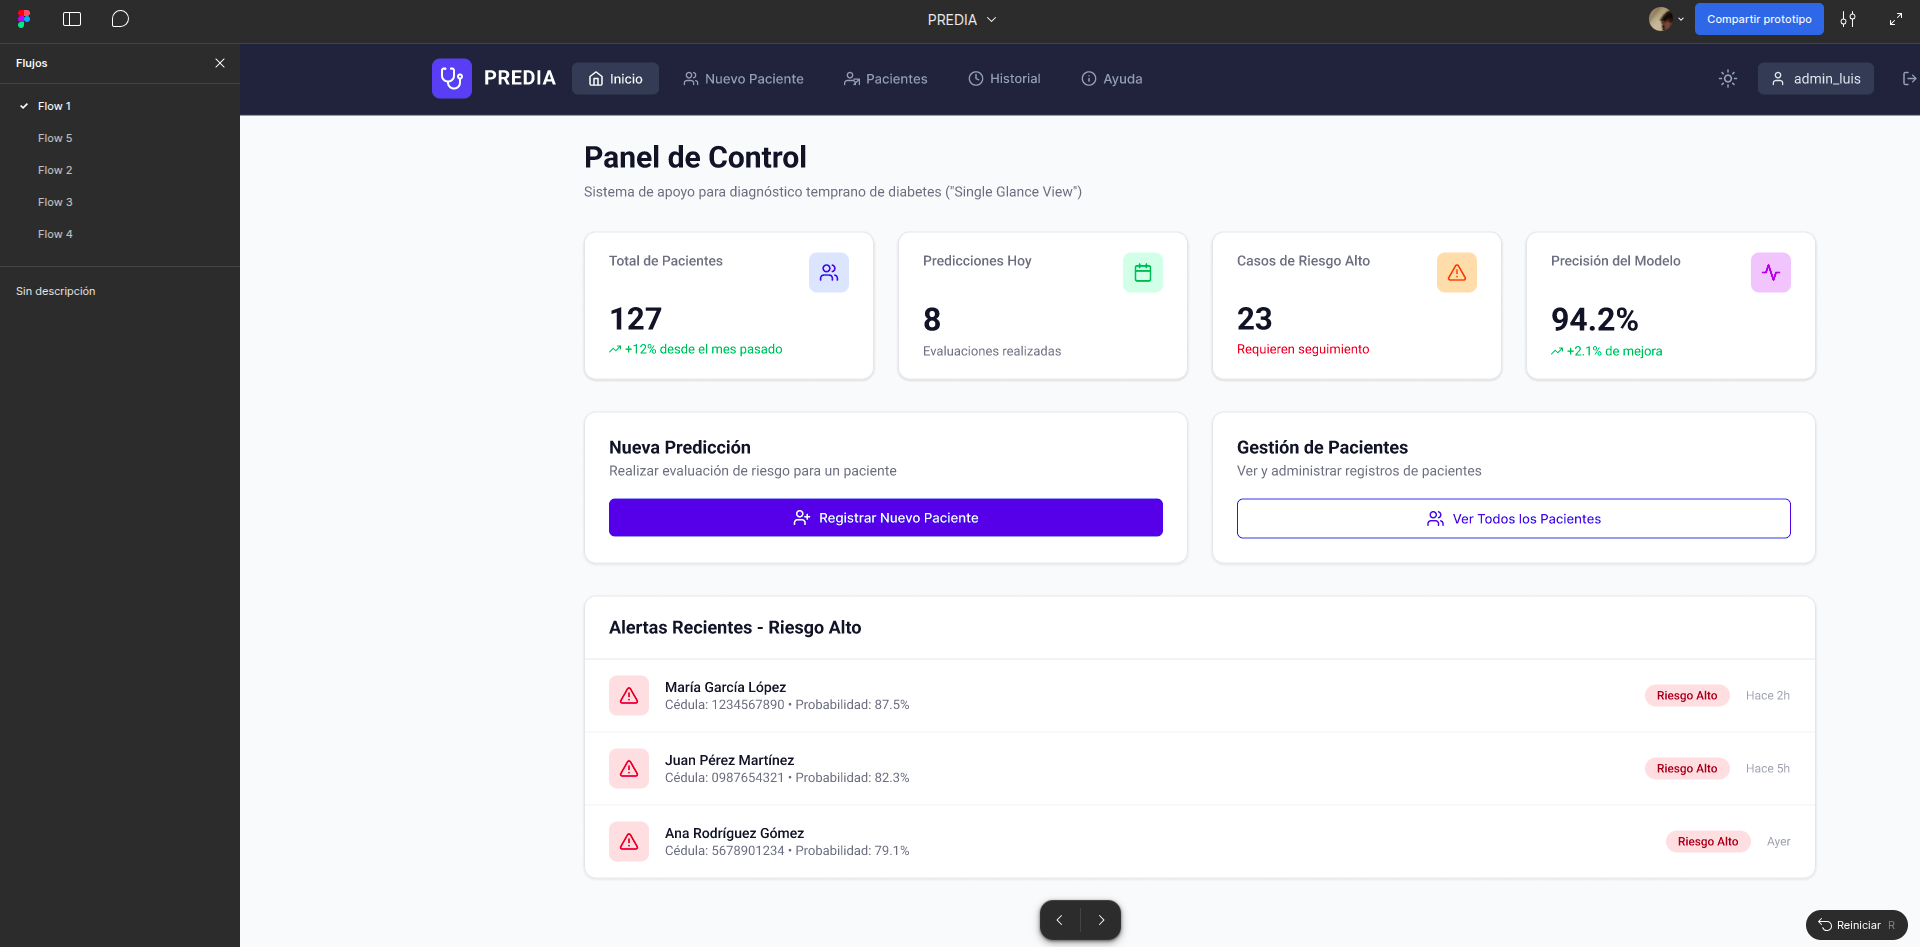
\includegraphics[width=0.85\linewidth]{img/mockup1.png}
  \caption{Desarrollo de los \textit{mockups} en Figma — Primera etapa.}
  \label{fig:mockup1}
\end{figure}

\subsubsection{Administración de proyectos de TI}

\textit{Entregable 1:} Acta de Constitución del Proyecto. \quad \textit{Estado:} \textbf{Completado.}

\smallskip
Información documentada:
\begin{itemize}[leftmargin=1.5cm]
  \item \textbf{Nombre del proyecto:} Predia — Plataforma Clínica Inteligente para la Detección Temprana de Diabetes.
  \item \textbf{Integrantes:} Giannoccaro Quiñonez A.\,V., Soriano Vega E.\,T., Álvarez Sánchez G., Muñoz Prado C.\,Y., Villafuerte Armenta G.\,I.
  \item \textbf{Objetivo SMART:} Plataforma con modelo IA de predicción de diabetes con $\geq$85\% precisión, $<$3~s tiempo de respuesta, 100+ usuarios concurrentes, en 12 meses de desarrollo bajo metodología Scrum.
  \item \textbf{Presupuesto:} CAPEX \$1{,}126{,}920 MXN; OPEX \$336{,}000 MXN/año.
  \item \textbf{Principales hitos:} Sistema base (Mes~2), Modelo IA integrado (Mes~4), Optimización (Mes~5), \textit{Testing} (Mes~7), Certificación ISO (Mes~12).
\end{itemize}

\textit{Entregable 2:} Caso de Negocio. \quad \textit{Estado:} \textbf{Completado.}

\begin{itemize}[leftmargin=1.5cm]
  \item \textbf{Evaluación financiera:} ROI 429.86\%, \textit{Payback} 1 año y 2 meses, VAN \$2{,}633{,}686.52 MXN.
\end{itemize}

\textit{Entregable 3:} Plan de Gestión de Recursos Humanos. \quad \textit{Estado:} \textbf{Completado.}

\begin{itemize}[leftmargin=1.5cm]
  \item Arianna Giannoccaro: Gerente del proyecto, desarrolladora BD.
  \item Elena Soriano: Analista/Desarrolladora APIs.
  \item Christopher Muñoz: Gestión técnica, analista de requisitos.
  \item Guillermo Álvarez: Desarrollador IA, \textit{Tester}.
  \item Gabriel Villafuerte: \textit{Full Stack}, \textit{Tester}.
\end{itemize}

%------------------------------------------------------------------------------
\subsection{Segunda etapa}

\subsubsection{Diseño de interfaces}

\textit{Entregable:} Video del prototipo con Figma. \quad \textit{Estado:} \textbf{Completado.}

\smallskip
Se completó el video demostrativo del prototipo navegable, y el \textit{frontend} fue desarrollado íntegramente en React~19 con Tailwind CSS. En esta etapa, la interfaz funcional quedó implementada y conectada con el \textit{backend}, superando la fase de prototipado.

\begin{figure}[H]
  \centering
  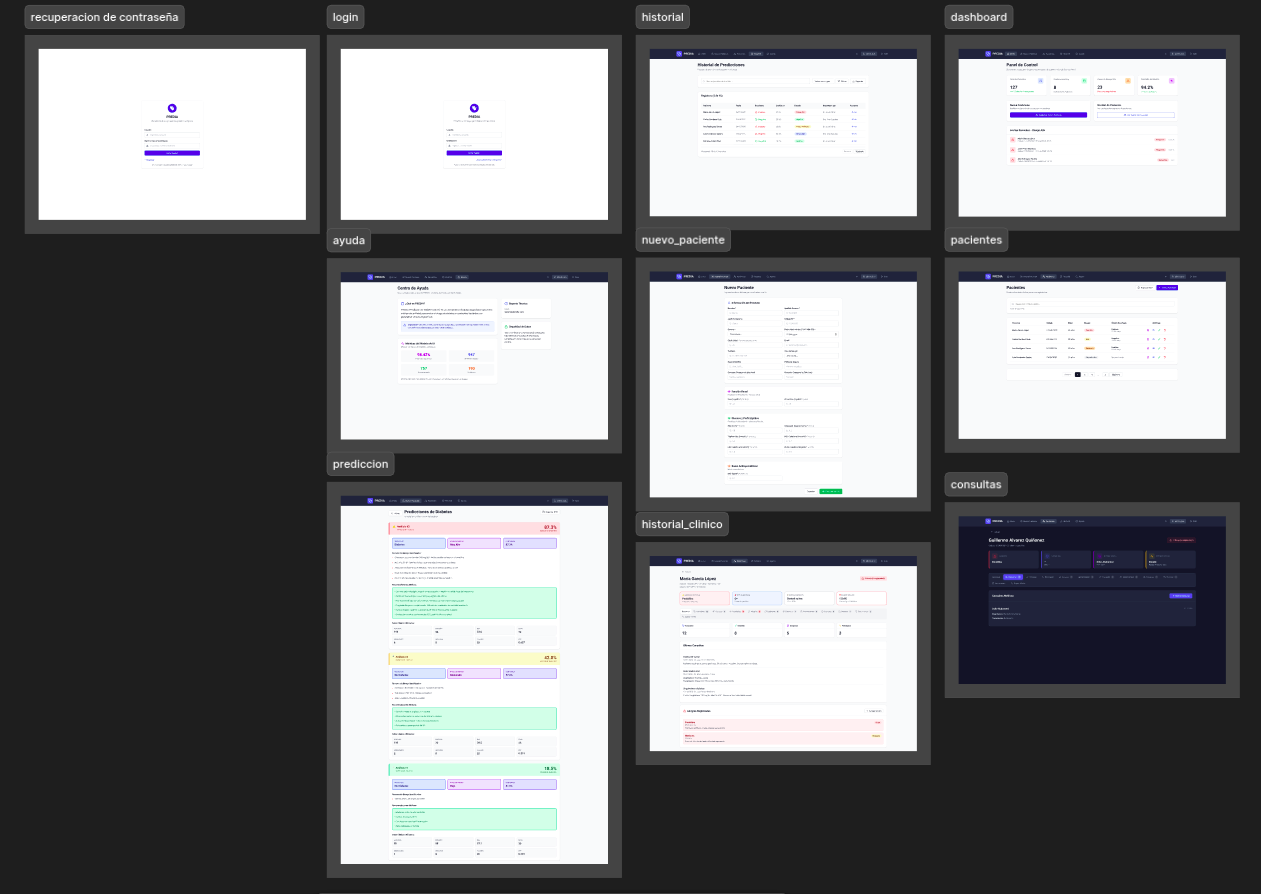
\includegraphics[width=0.88\linewidth]{img/mockup2.png}
  \caption{Prototipo funcional de PREDIA — Segunda etapa.}
  \label{fig:mockup2}
\end{figure}

\subsubsection{Tecnologías de virtualización}

\textit{Entregable:} Despliegue funcional + Documentación. \quad \textit{Estado:} \textbf{Completado.}

El sistema completo fue desplegado mediante Docker y Docker Compose, integrando los tres componentes principales: el \textit{frontend} con Next.js, el \textit{backend} con API REST y la base de datos MySQL~10.11.13. Se configuraron volúmenes persistentes y se automatizó el proceso de inicialización mediante el \textit{script} \texttt{setup.sh}. La documentación de instalación y configuración se completó de manera integral.

\subsubsection{Tecnologías y aplicaciones en Internet}

\textit{Entregable:} Análisis y diseño del proyecto. \quad \textit{Estado:} \textbf{Completado.}

\smallskip
\textbf{Análisis:} Descripción de la solución, diagrama de flujo, requerimientos funcionales y no funcionales documentados.

\textbf{Diseño:} Casos de uso, diagramas de secuencia (flujos de predicción, autenticación, consultas), diagrama de componentes, diccionario de datos (11 modelos), diagrama relacional de BD, interfaces programadas en React, repositorio GitHub activo.

\subsubsection{Administración de proyectos de TI}

\textit{Entregable 1:} Plan de Gestión de Adquisiciones. \quad \textit{Estado:} \textbf{Completado.}

\begin{itemize}[leftmargin=1.5cm]
  \item Infraestructura: \$100{,}000 MXN para 5 equipos y servidor.
  \item Certificación ISO 13485: \$200{,}000--\$300{,}000 MXN.
  \item Capacitación ML: \$2{,}000 MXN.
\end{itemize}

\textit{Entregable 2:} Plan de Gestión de la Calidad. \quad \textit{Estado:} \textbf{Completado.}

\begin{itemize}[leftmargin=1.5cm]
  \item \textbf{Estándares:} NOM-015-SSA2-2010, NOM-151-SCFI-2016, NOM-241-SSA1-2025, LFPDPPP 2025, ISO 13485, WCAG 2.1 AA, OWASP Top 10.
  \item \textbf{KPIs:} Exactitud $\geq$85\% (97.89\% alcanzado), respuesta $<$3~s, \textit{uptime} $\geq$99.5\%, 0 vulnerabilidades críticas, cobertura $\geq$80\% (83.4\% alcanzado), SUS $\geq$70 (78.5 alcanzado).
  \item Estrategias de pruebas, criterios de aceptación, auditorías, checklists y matriz de defectos documentados.
\end{itemize}

\textit{Entregable 3:} Dirección y Gestión del Trabajo. \quad \textit{Estado:} \textbf{Completado.}

\begin{itemize}[leftmargin=1.5cm]
  \item WBS, bitácora de problemas y minutas implementadas según metodología Scrum documentada.
\end{itemize}

%------------------------------------------------------------------------------
\section{Análisis de los resultados}
%------------------------------------------------------------------------------

El análisis de resultados del proyecto PREDIA se realizó con base en el cumplimiento de los entregables establecidos en cada una de las materias involucradas, evaluando tanto el desempeño técnico del sistema como la integración global del proyecto.

\subsection{Tecnologías y aplicaciones en Internet}

El resultado principal fue la implementación de un sistema funcional basado en una arquitectura desacoplada, cumpliendo con la separación entre \textit{frontend}, \textit{backend}, API y base de datos. Se logró implementar más de 24 endpoints REST, dos módulos CRUD completos (gestión de pacientes y registros clínicos) y dashboards con gráficas dinámicas. Asimismo, se desarrolló la funcionalidad de generación de reportes en formato PDF con información clínica y resultados del modelo de ML.

De manera crítica, la integración con estándares de interoperabilidad médica (como HL7 FHIR) aún no ha sido validada en escenarios reales, lo que representa una oportunidad de mejora.

\subsection{Tecnologías de virtualización}

Se logró la implementación completa del sistema dentro de un entorno virtualizado con Docker y Docker Compose, incluyendo todos los componentes: frontend, backend, base de datos y servicios asociados. La documentación generada detalla el proceso de instalación, configuración y ejecución del sistema. Sin embargo, se identificó que no se realizaron pruebas extensivas de rendimiento en entornos de alta concurrencia, limitando la validación completa de la escalabilidad.

\subsection{Diseño de interfaces}

Las interfaces fueron desarrolladas utilizando React y Next.js, logrando una integración efectiva con la API REST. El sistema presenta dashboards diferenciados por rol, formularios de captura de datos clínicos y visualización de resultados de predicción. El puntaje de usabilidad obtenido (SUS 78.5) indica una experiencia de usuario adecuada. Se identificó como limitación la falta de adaptación a dispositivos móviles.

\subsection{Administración de proyectos de TI}

El proyecto se desarrolló dentro del tiempo estimado mediante la metodología Scrum. Se presentaron bloqueos relacionados con la integración del modelo de IA y la validación de datos, gestionados sin afectar significativamente el avance general. El presupuesto inicial fue suficiente para cubrir los requerimientos del proyecto. En las lecciones aprendidas, se identificaron aspectos positivos como la correcta integración entre materias y el uso de tecnologías modernas, así como áreas de mejora, incluyendo la necesidad de mayor validación de datos y pruebas en entornos reales.

\subsection{Análisis global del sistema}

En términos globales, PREDIA cumple con los requisitos funcionales y técnicos establecidos, logrando una integración efectiva entre las diferentes áreas disciplinares que conforman el proyecto. El sistema opera como una solución cohesiva que articula gestión clínica, visualización de datos y predicción mediante inteligencia artificial.

No obstante, el análisis también permite identificar limitaciones relevantes que condicionan el alcance actual de la plataforma: la validación del sistema no se ha realizado en entornos clínicos reales, las pruebas de escalabilidad bajo alta concurrencia están pendientes, y el modelo de \textit{Machine Learning} depende de un \textit{dataset} de 757 muestras, cuyo tamaño limitado puede incidir tanto en posibles sesgos como en la capacidad de generalización del modelo. Estas áreas representan oportunidades críticas de mejora para la evolución futura de la plataforma.

%=============================================================================
\chapter{Conclusiones}
%=============================================================================

El desarrollo del proyecto PREDIA permitió integrar de manera efectiva conocimientos de diversas áreas de la ingeniería de software en una solución tecnológica orientada al sector salud. A lo largo del proyecto se abordaron problemáticas concretas relacionadas con la detección tardía de la diabetes y la gestión ineficiente de historiales clínicos, proponiendo una plataforma que articula funcionalidades de gestión médica con capacidades predictivas basadas en inteligencia artificial.

En relación con los objetivos específicos planteados, los resultados obtenidos permiten afirmar que se alcanzó un cumplimiento satisfactorio en la mayoría de ellos. El sistema integral de gestión de información clínica (OE1) se implementó con operaciones CRUD completas y validación automática conforme a la NOM-015-SSA2-2010. El módulo de captura de datos clínicos estructurados (OE2) incorpora los rangos de validación definidos y alertas visuales. El modelo de Inteligencia Artificial (OE3) alcanzó una exactitud del 97.89\% ---superior al mínimo del 85\% requerido---, con predicciones en menos de 3 segundos y explicabilidad de los 5 factores principales, aunque su validación con poblaciones clínicas diversas permanece pendiente. La interfaz de usuario (OE4) obtuvo un puntaje SUS de 78.5 con cumplimiento WCAG~2.1 nivel~AA y diseño \textit{responsive} para \textit{desktop} y tabletas. El sistema de reportes (OE5) genera documentos PDF en el tiempo requerido con la información clínica especificada.

Desde el punto de vista técnico, el sistema evidencia una implementación adecuada de una arquitectura desacoplada basada en API REST, la cual facilita la comunicación entre los distintos componentes (\textit{frontend}, \textit{backend}, base de datos y modelo de inteligencia artificial). La selección de tecnologías como Next.js, MySQL y Docker ---cuya justificación se aborda en el marco teórico--- permitió construir una solución mantenible y alineada con las prácticas actuales de desarrollo de software.

El impacto potencial del sistema en el contexto clínico radica en su capacidad para apoyar la detección temprana de la diabetes, proporcionando al personal médico una herramienta complementaria ---no sustitutiva--- para la toma de decisiones. La centralización de la información clínica, junto con la generación de reportes y la visualización de datos mediante \textit{dashboards}, contribuye a mejorar la organización y el análisis de la información del paciente.

No obstante, el proyecto presenta limitaciones que deben abordarse con transparencia. El modelo de \textit{Machine Learning} fue entrenado con un conjunto de 757 muestras, un tamaño que, si bien permitió obtener métricas favorables, limita la confianza en la generalización del modelo a poblaciones clínicas heterogéneas y plantea el riesgo de sobreajuste. Además, el sistema no ha sido sometido a validación en un entorno clínico real, lo que impide confirmar su efectividad en condiciones de uso práctico. En términos de infraestructura, la ausencia de pruebas extensivas bajo escenarios de alta concurrencia constituye una limitación adicional en cuanto a la verificación de su escalabilidad.

A partir de estas observaciones, se identifican líneas de trabajo futuro prioritarias: ampliar el \textit{dataset} de entrenamiento con mayor diversidad demográfica y clínica, realizar validaciones en colaboración con profesionales de la salud en entornos reales, ejecutar pruebas de carga para verificar la escalabilidad, extender la compatibilidad a dispositivos móviles, y avanzar en el cumplimiento de certificaciones que respalden el uso del sistema en el sector salud.

En síntesis, PREDIA constituye una solución viable desde las perspectivas técnica y académica, y demuestra la capacidad de integrar múltiples disciplinas en un proyecto funcional con aplicabilidad real. Su transición hacia un entorno productivo dependerá de un proceso sostenido de validación clínica, ampliación del conjunto de datos, mejora continua y cumplimiento normativo, lo cual define un horizonte claro de investigación y desarrollo en el ámbito de la salud digital.

%=============================================================================
% REFERENCIAS Y BIBLIOGRAFÍA
%=============================================================================
%\bibliographystyle{apalike}
%\bibliography{referencias}

%=============================================================================
% BIBLIOGRAFÍA COMPLETA (entrada manual como alternativa)
%=============================================================================
\cleardoublepage
\phantomsection
\addcontentsline{toc}{chapter}{Bibliografía}

% Si no se usa archivo .bib, descomentar y usar \begin{thebibliography}

\begin{thebibliography}{99}

\bibitem{barquera2021}
Barquera, S., Hernández-Alcaraz, C., Jáuregui, A., Medina, C., Mendoza-Herrera, K., Pedroza-Tobias, A., \ldots\ \& Aguilar Salinas, C.~A. (2021). Diabetes awareness, treatment, and control among Mexico City residents. \textit{Diabetology, 2}(1), 16--30. \url{https://doi.org/10.3390/diabetology2010002}

\bibitem{basto2021}
Basto-Abreu, A., López-Olmedo, N., Rojas-Martínez, R., Aguilar-Salinas, C.~A., de la Cruz-Góngora, V., Rivera-Dommarco, J., \ldots\ \& Barrientos-Gutiérrez, T. (2021). Prevalence of diabetes and glycemic control in Mexico: National results from 2018 and 2020. \textit{Salud Pública de México, 63}(6), 725--733. \url{https://doi.org/10.21149/12842}

\bibitem{beam2018}
Beam, A.~L., \& Kohane, I.~S. (2018). Big data and machine learning in health care. \textit{JAMA, 319}(13), 1317--1318. \url{https://doi.org/10.1001/jama.2017.18391}

\bibitem{contreras2018}
Contreras, I., \& Vehi, J. (2018). Artificial intelligence for diabetes management and decision support: Literature review. \textit{Journal of Medical Internet Research, 20}(5), e10775. \url{https://doi.org/10.2196/10775}

\bibitem{idf_atlas}
International Diabetes Federation. (s.f.). \textit{Mexico diabetes statistics \& prevalence}. IDF Diabetes Atlas. \url{https://diabetesatlas.org/data-by-location/country/mexico/}

\bibitem{kavakiotis2017}
Kavakiotis, I., Tsave, O., Salifoglou, A., Maglaveras, N., Vlahavas, I., \& Chouvarda, I. (2017). Machine learning and data mining methods in diabetes research. \textit{Computational and Structural Biotechnology Journal, 15}, 104--116. \url{https://doi.org/10.1016/j.csbj.2016.12.005}

\bibitem{lfpdppp2025}
Comisión Nacional de Protección y Defensa de los Usuarios de Servicios Financieros. (2025). \textit{Ley Federal de Protección de Datos Personales en Posesión de los Particulares} [Actualización 2025]. Diario Oficial de la Federación.

\bibitem{nom015}
Diario Oficial de la Federación. (2010, 23 de noviembre). \textit{NOM-015-SSA2-2010, Para la prevención, tratamiento y control de la diabetes mellitus}. \url{https://www.dof.gob.mx/normasOficiales/4215/salud/salud.htm}

\bibitem{ogle2025}
Ogle, G.~D., Wang, F., Haynes, A., Gregory, G.~A., King, T.~W., Deng, K., \ldots\ \& Maniam, J. (2025). Global type 1 diabetes prevalence, incidence, and mortality estimates 2025. \textit{Diabetes Research and Clinical Practice, 225}, Artículo 112277. \url{https://doi.org/10.1016/j.diabres.2025.112277}

\bibitem{rodriguez2019}
Rodríguez-Rodríguez, I., Chatzigiannakis, I., Rodríguez, J.~V., Maranghi, M., Gentili, M., \& Zamora-Izquierdo, M.~Á. (2019). Utility of big data in predicting short-term diabetes progression using machine learning. \textit{Electronics, 8}(11), Artículo 1364. \url{https://doi.org/10.3390/electronics8111364}

\end{thebibliography}

%=============================================================================
% ANEXOS
%=============================================================================
\appendix
\chapter{Anexo}

\textit{[Contenido por completar.]}

%=============================================================================
\end{document}